\documentclass[12pt]{article}

%---------------------------------
%中文设置
\usepackage[UTF8]{ctexcap}
\setCJKsansfont[ItalicFont={黑体}]{宋体}
\renewcommand\CJKfamilydefault{\CJKsfdefault}
\setCJKmonofont{仿宋}

%英文字体
\setmainfont{Times New Roman}


\renewcommand{\figurename}{图}
\renewcommand{\contentsname}{目录}
\renewcommand{\abstractname}{摘要}
\renewcommand{\refname}{参考文献}
\setlength{\parindent}{3em}
%图表标题设置
\usepackage[margin=9pt, font=small, labelfont=bf,labelsep=quad]{caption}[2012/03/25 v3.3]

%中英双标题
%\bicaption{中文标题}{English title}
% \usepackage{bicaption}[2012/04/09 v1.1]

% \captionsetup[figure][bi-first]{name=图}
% \captionsetup[figure][bi-second]{name=Figure}

% \captionsetup[table][bi-first]{name=表}
% \captionsetup[table][bi-second]{name=Table}

%----------------------------------
% enumerate setting
\usepackage{enumitem}
%----------------------------------
%页面设置
%使\section中的内容左对齐
\usepackage[raggedright]{titlesec}

\setcounter{secnumdepth}{4}

\titleformat{\paragraph}
{\normalfont\normalsize\bfseries}{\theparagraph}{1em}{}
\titlespacing*{\paragraph}
{0pt}{3.25ex plus 1ex minus .2ex}{1.5ex plus .2ex}

%页眉页脚
%\usepackage{fancyhdr}
%\pagestyle{fancy}
%\fancyhead[L]{}
%\fancyhead[R]{}

%页边距
\usepackage{geometry}
\geometry{left=2cm,right=2cm,top=2.5cm,bottom=2.5cm}

%---------------------------------
%matlab代码显示
%\usepackage[framed,numbered,autolinebreaks,useliterate]{mcode}

%---------------------------------
%数学符号显示
\usepackage{amssymb}
\usepackage{amsmath}
\usepackage{bm}

%---------------------------------
%罗马数字定义
\makeatletter
\newcommand{\rmnum}[1]{\romannumeral #1}
\newcommand{\Rmnum}[1]{\expandafter\@slowromancap\romannumeral #1@}
\makeatother

%\renewcommand{\labelenumi}{\roman{enumi}}

%---------------------------------
%方程组
%\begin{equation}
%   \left\{
%   \begin{aligned}
%       &x_2 =0\\
%       &x_1 =0\\
%       &x_1 =1\\
%       &x_2(1-x_1)^4 =1
%   \end{aligned}
%   \right.
%\end{ }

%---------------------------------
%插图
\usepackage{graphicx}
\usepackage{emp}

%文字绕排
\usepackage{wrapfig}
%\begin{wrapfigure}[<行数>]{<位置>l/r}[<外伸长度>}]{<宽度>}
%   \centering
%   \caption{ }
%   \includegraphics[ ]{ }
%\end{ }

%双图
%\begin{figure}
%   \centering
%   \caption{ }
%   \includegraphics[ ]{ }
%       \subcaption{ }
%   \qquad
%   \includegraphics[ ]{ }
%       \subcaption{ }
%\end{ }

%---------------------------------
%标题
\usepackage{caption, subcaption}
%\captionsetup{font = {small, sf}, labelfont = bf}
%字号选择:
%- scriptsize
%- footnotesize
%- small
%- normalsize
%- large
%- Large
%
%字体族:
%- rm 罗马体
%- sf 无衬线体
%- tt 打字机体
%
%字体系列:
%- md 中等粗细
%- bf 粗体
%
%字体形状:
%- up 直立体
%- it 意大利体
%- sl 倾斜体
%- sc 小型大写字母

%---------------------------------
%表格
\usepackage{longtable}
\usepackage{booktabs}
\usepackage{bigstrut}
\usepackage{multirow}
\usepackage{array}
\usepackage[table]{xcolor}
\usepackage{tikz}
\usepackage{chngpage}
%\begin {table}[H]
%\caption{This is a long table}
%\begin{adjustwidth}{-3cm}{} %第一个参数为调整左页边距,第二个参数右页边距可置空
%\end{adjustwidth}
%\end{table}

\usepackage{import}
\usepackage{authblk}

\newcommand{\specialcell}[2][l]{%
     \begin{tabular}[#1]{@{}l@{}}#2\end{tabular}}


%---------------------------------
\def\tightlist{}

%---------------------------------
\begin{document}

\title{ \textbf{\emph{Java大作业选题报告}}}
\date{\today}
\author{王超杰 ~ ~ 学号:2013010179 \\ 林超超 ~ ~ 学号:2013010199}

\maketitle

%---------------------------------
% \abstract

%\thispagestyle{empty}
%\newpage
\tableofcontents
\thispagestyle{empty}
\newpage
\setcounter{page}{1}

%---------------------------------

\section{现有todo类应用}
% \label{sec:现有todo类应用}
    \subsection{Todoist}
    \label{sub:Todoist}

        Todoist是笔者最初使用的todo类应用。它支持project、label、filter等todo类应用的标准功能,且premium版本(一年199元,如果在Google play上用美元支付,折算成大约在160-180元人民币之间)允许用户自定义filter,查找、定位任务非常方便,且premium版本支持用户在任务中添加附件,如pdf等。UI采用标准的material design,非常简洁美观(图\ref{fig:design})。此外,Todoist号称全平台(除Linux)通用,甚至推出了功能强大的官方Gmail插件,可以直接从Gmail中创建任务,并把附件添加到任务说明中。各个平台的同步速度都非常快,没有出现国外软件常见的服务器架设在国外导致同步龟速的现象。Todoist还有独特的Karma值系统(图\ref{fig:karma}),根据用户每天完成任务的数量和质量进行积分累计,premium版本可以对自己每天完成任务的情况进行跟踪,非常有利于不断提升自己的工作效率。

        \begin{figure}[htbp]
            \centering
            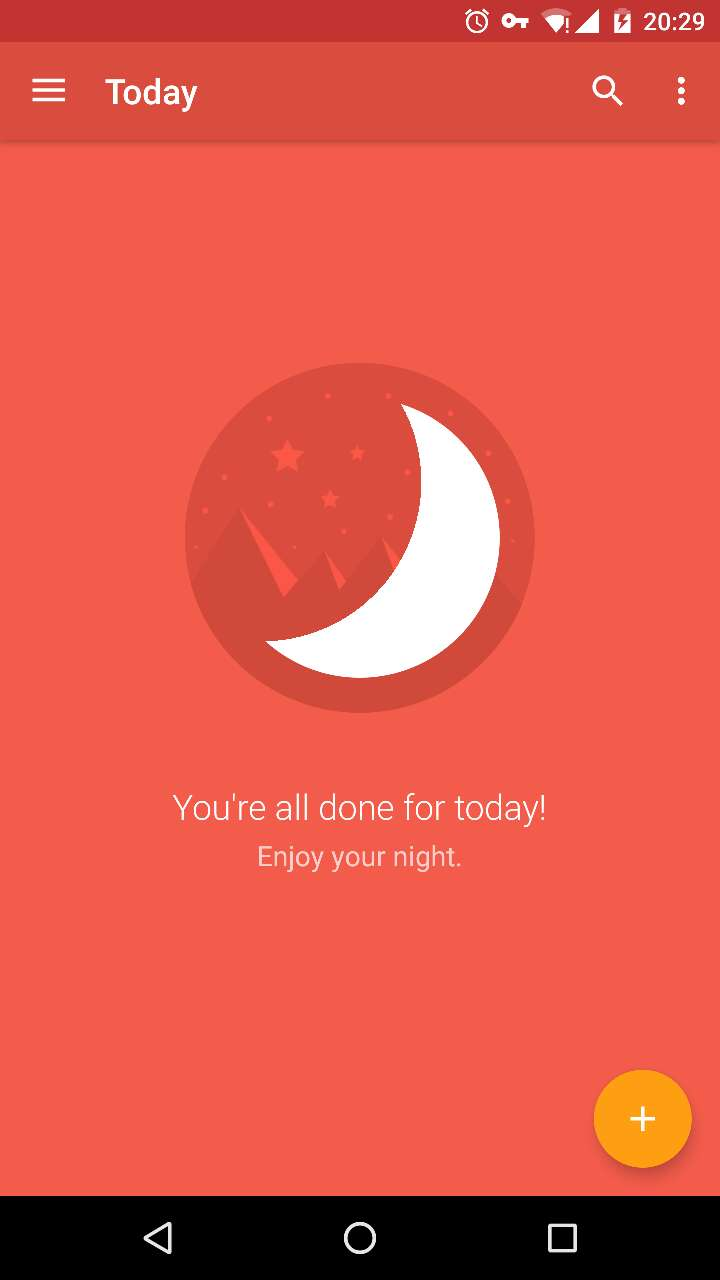
\includegraphics[width=0.4\textwidth]{figure/design}
            \caption{Material Design Code}
            \label{fig:design}
        \end{figure}

        \begin{figure}[htbp]
            \centering
            
\includegraphics[width=0.7\textwidth]{figure/karma}
            \caption{Karma值2605}
            \label{fig:karma}
        \end{figure}

        但是,Todoist在以下三个方面不能满足我的使用需求:
        \begin{itemize}
            \item 无defer功能

                defer是GTD(Get Things Done)中非常重要的一环,指任务现在缺乏一些必要条件无法着手进行,必须推迟到未来处理,例如你可能现在就知道自己要准备java期末考试的复习,但现在是第八周,课程都还没有学完,复习的条件不满足。如果你把它写到待办事项里,会给自己造成很大压力,且在决定做哪项任务时让人分心,因为它每天都呆在那里,可是由于非主观的原因你又无法完成它。所以这时候我们应该选择把它推迟到16周周末,这样在第8-16周我们都不会看到它了,但到16周周末时它又会及时提醒我们要复习java。

                目前android平台上的todo类应用均没有defer功能。但就在上周google calendar推出了一项全新功能:goals。它允许用户设定目标,并为用户自动规划和安排时间,这个时间允许用户推迟。但这个推迟不允许用户手动调整,是google通过机器学习算法自动安排的,而且从严格意义上讲,这不是todo类应用,因为这些goals是整体目标,例如学英语、学编程等,不是一个“代办事项”。

                IOS平台上的OmniFocus则很好地实现了defer的功能,但其没有Android版本,也没有开放API。实际上Omni Group只有为IOS和Mac设计的产品。

            \item 不支持项目的无限层级

                \begin{figure}[htbp]
                    \centering
                    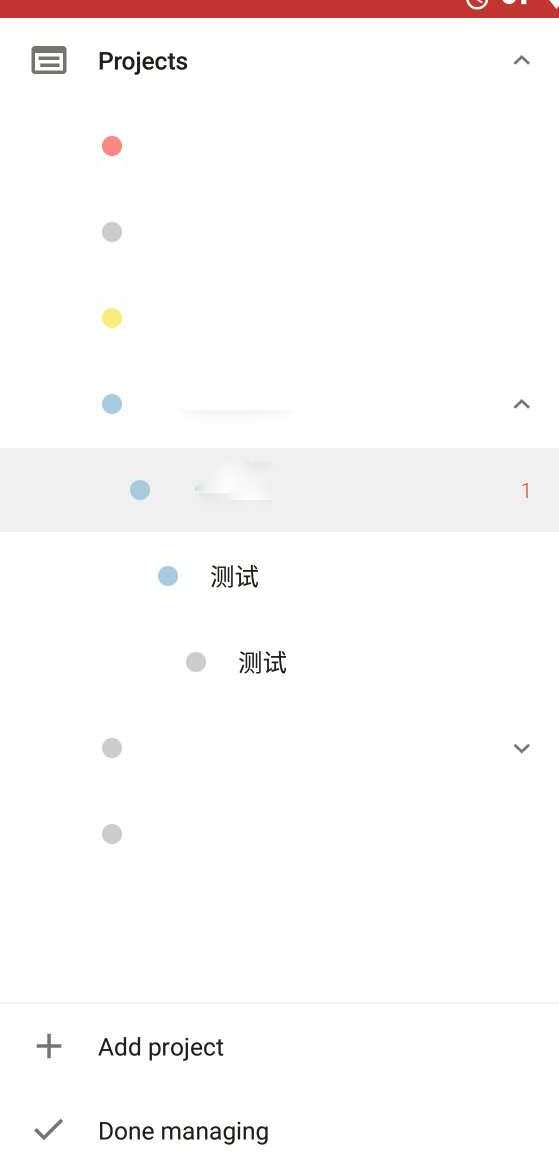
\includegraphics[height=0.3\textheight]{figure/quar}
                    \caption{最多支持四个子项目}
                    \label{fig:quar}
                \end{figure}

                有时候我们的任务是非常复杂的。比如java考试作为一个project,它范围太大,让人无从下手。或许我们可以为它设置一个二级子任务叫类,再设置一个三级子任务叫package的应用,然后可能还需要设置四级子任务叫java基础类库。但我们可能还需要再细化到某一个具体的包,因为java基础类库种类还是太多了。于是我们想再设置五级子任务,譬如java.lang。但Todoist只支持四级子任务,不能无限分级。

            \item 价格

                和动辄两三百元的OmniFocus相比,年费199元看上去很划算,但Todo类应用用户的黏着性大,用上十年这笔开销都够买Omni Focus, Omni Graffle, Omni Outliner, Omni Plan, Omni Presence总之就是Omni Group的全家桶了。
        \end{itemize}

    \subsection{Wunderlist}
    \label{sub:Wunderlist}
        Wunderlist是近年很火的todo应用,后被Microsoft收购。笔者只是对其进行了简单测试,发现了以下几点不能让笔者满意的地方:

        \begin{itemize}
            \item 又是价格

                Wunderlist更贵,pro版本年费49.99刀,人民币估计在300元左右。这样算起来用上十年可以买一堆正版的生产力软件了。

            \item 不支持地点提醒

                Wunderlist不支持根据所在地点推送提醒。比如有些事情我可能需要在宿舍才能完成,那么这些事情就不应该按照时间来提醒,而应该根据我目前的位置来向我推送通知。Todoist和OmniFocus的IOS版本均支持,但Wunderlist不支持。

            \item 没有标签

                没有标签意味着无法将处于不同项目下、但又具有某些相同特点的任务聚类同时处理。比如假设我这学期同时上郑老师的Java和C++课,根据正常人的理解都会把Java和C++设置成两个项目,然后Java和C++的问题各自写在各自的项目里。问题来了,当我有机会向郑老师或者助教请教问题时,我需要查找两个项目才能找到所有的问题,假设郑老师同时开设Python, HTML5, C\#, Fortran...呢?所以这时候我需要给我这些不同的问题贴上一个共同的标签,不妨就叫做“郑老师”,那么当我遇到郑老师时,我只要查找“郑老师”这个标签就可以找到郑老师讲授的所有课程的问题了。如果说项目像是Tree结构一样,提供的是垂直的视角,标签则给这棵树提供了一个横向的查看类似的node的视角。

        \end{itemize}

    \subsection{Google Keep}
    \label{sub:Google Keep}
        Google Keep是笔者非常喜欢的一个轻量级Note类应用,也能通过checkbox提供基本的todo应用功能。作为Google自家应用,UI设计自然是Material Design的典范。与Google calendar或Inbox by Gmail共同使用时,可以方便地将待办事项整合进Google calendar中,非常方便。且借助于google强大的Machine Learning系统(以及它掌握的大量关于我们的私人数据),Google Keep甚至可以在你输入任务时给出autocompletion,虽然感觉其中涉及到很多privacy的问题非常creepy,但的确是生产力大杀器。而且Google Keep麻雀虽小五脏俱全,同时支持标签、定时提醒、地点提醒等功能。不过,作为轻量级应用,Google Keep没有项目的概念,而是通过标签来管理,这在管理大型项目时非常不方便。同时,Google Keep也不支持defer功能。


%---------------------------------
%参考文献

\bibliographystyle{plain}
% \bibliography{bibtex/report}

%---------------------------------
\end{document}
